\documentclass[12pt]{standalone}
\usepackage{cmbright}
\usepackage[T1]{fontenc}
\usepackage{tikz}
\usepackage{pgfplots}
\usetikzlibrary{shapes.geometric, positioning, calc, shadings}
  \tikzset{%
  db/.style = {cylinder, draw, fill=white, inner sep=2pt},
  tool/.style = {rectangle, draw, fill=white, inner sep=2pt},
  data/.style = {},
  func/.style = {},
  fake/.style = {},
  path/.style = {thick},
  dna/.style = {draw, very thick},
  pipe/.style = {draw, very thick, dashed},
  partLabel/.style = {font=\bfseries,
                      fill=gray!10,rounded corners, draw=black!50, dashed},
  every legend to name picture/.style={west}
  }
  \pgfdeclareplotmark{db}{\node [cylinder, draw=black] {};}

  \definecolor{struc}{rgb}{0.8,0.09,0.01}
  \definecolor{func}{rgb}{0.17,0.48,0.71}
  \definecolor{rightfl}{rgb}{0.14,0.75,0.4}
  \definecolor{leftfl}{rgb}{0.64,0.06,0.06}

%% https://tex.stackexchange.com/questions/62262/legend-in-tikzpicture
% argument #1: any options
\newenvironment{customlegend}[1][]{%
    \begingroup
    % inits/clears the lists (which might be populated from previous
    % axes):
    \csname pgfplots@init@cleared@structures\endcsname
    \pgfplotsset{#1}%
}{%
    % draws the legend:
    \csname pgfplots@createlegend\endcsname
    \endgroup
}%

% makes \addlegendimage available (typically only available within an
% axis environment):
\def\addlegendimage{\csname pgfplots@addlegendimage\endcsname}

%%--------------------------------

% definition to insert numbers
\pgfkeys{/pgfplots/number in legend/.style={%
        /pgfplots/legend image code/.code={%
            \node at (0.125,-0.0225){#1}; % <= changed x value
        },%
    },
}
\begin{document}
  -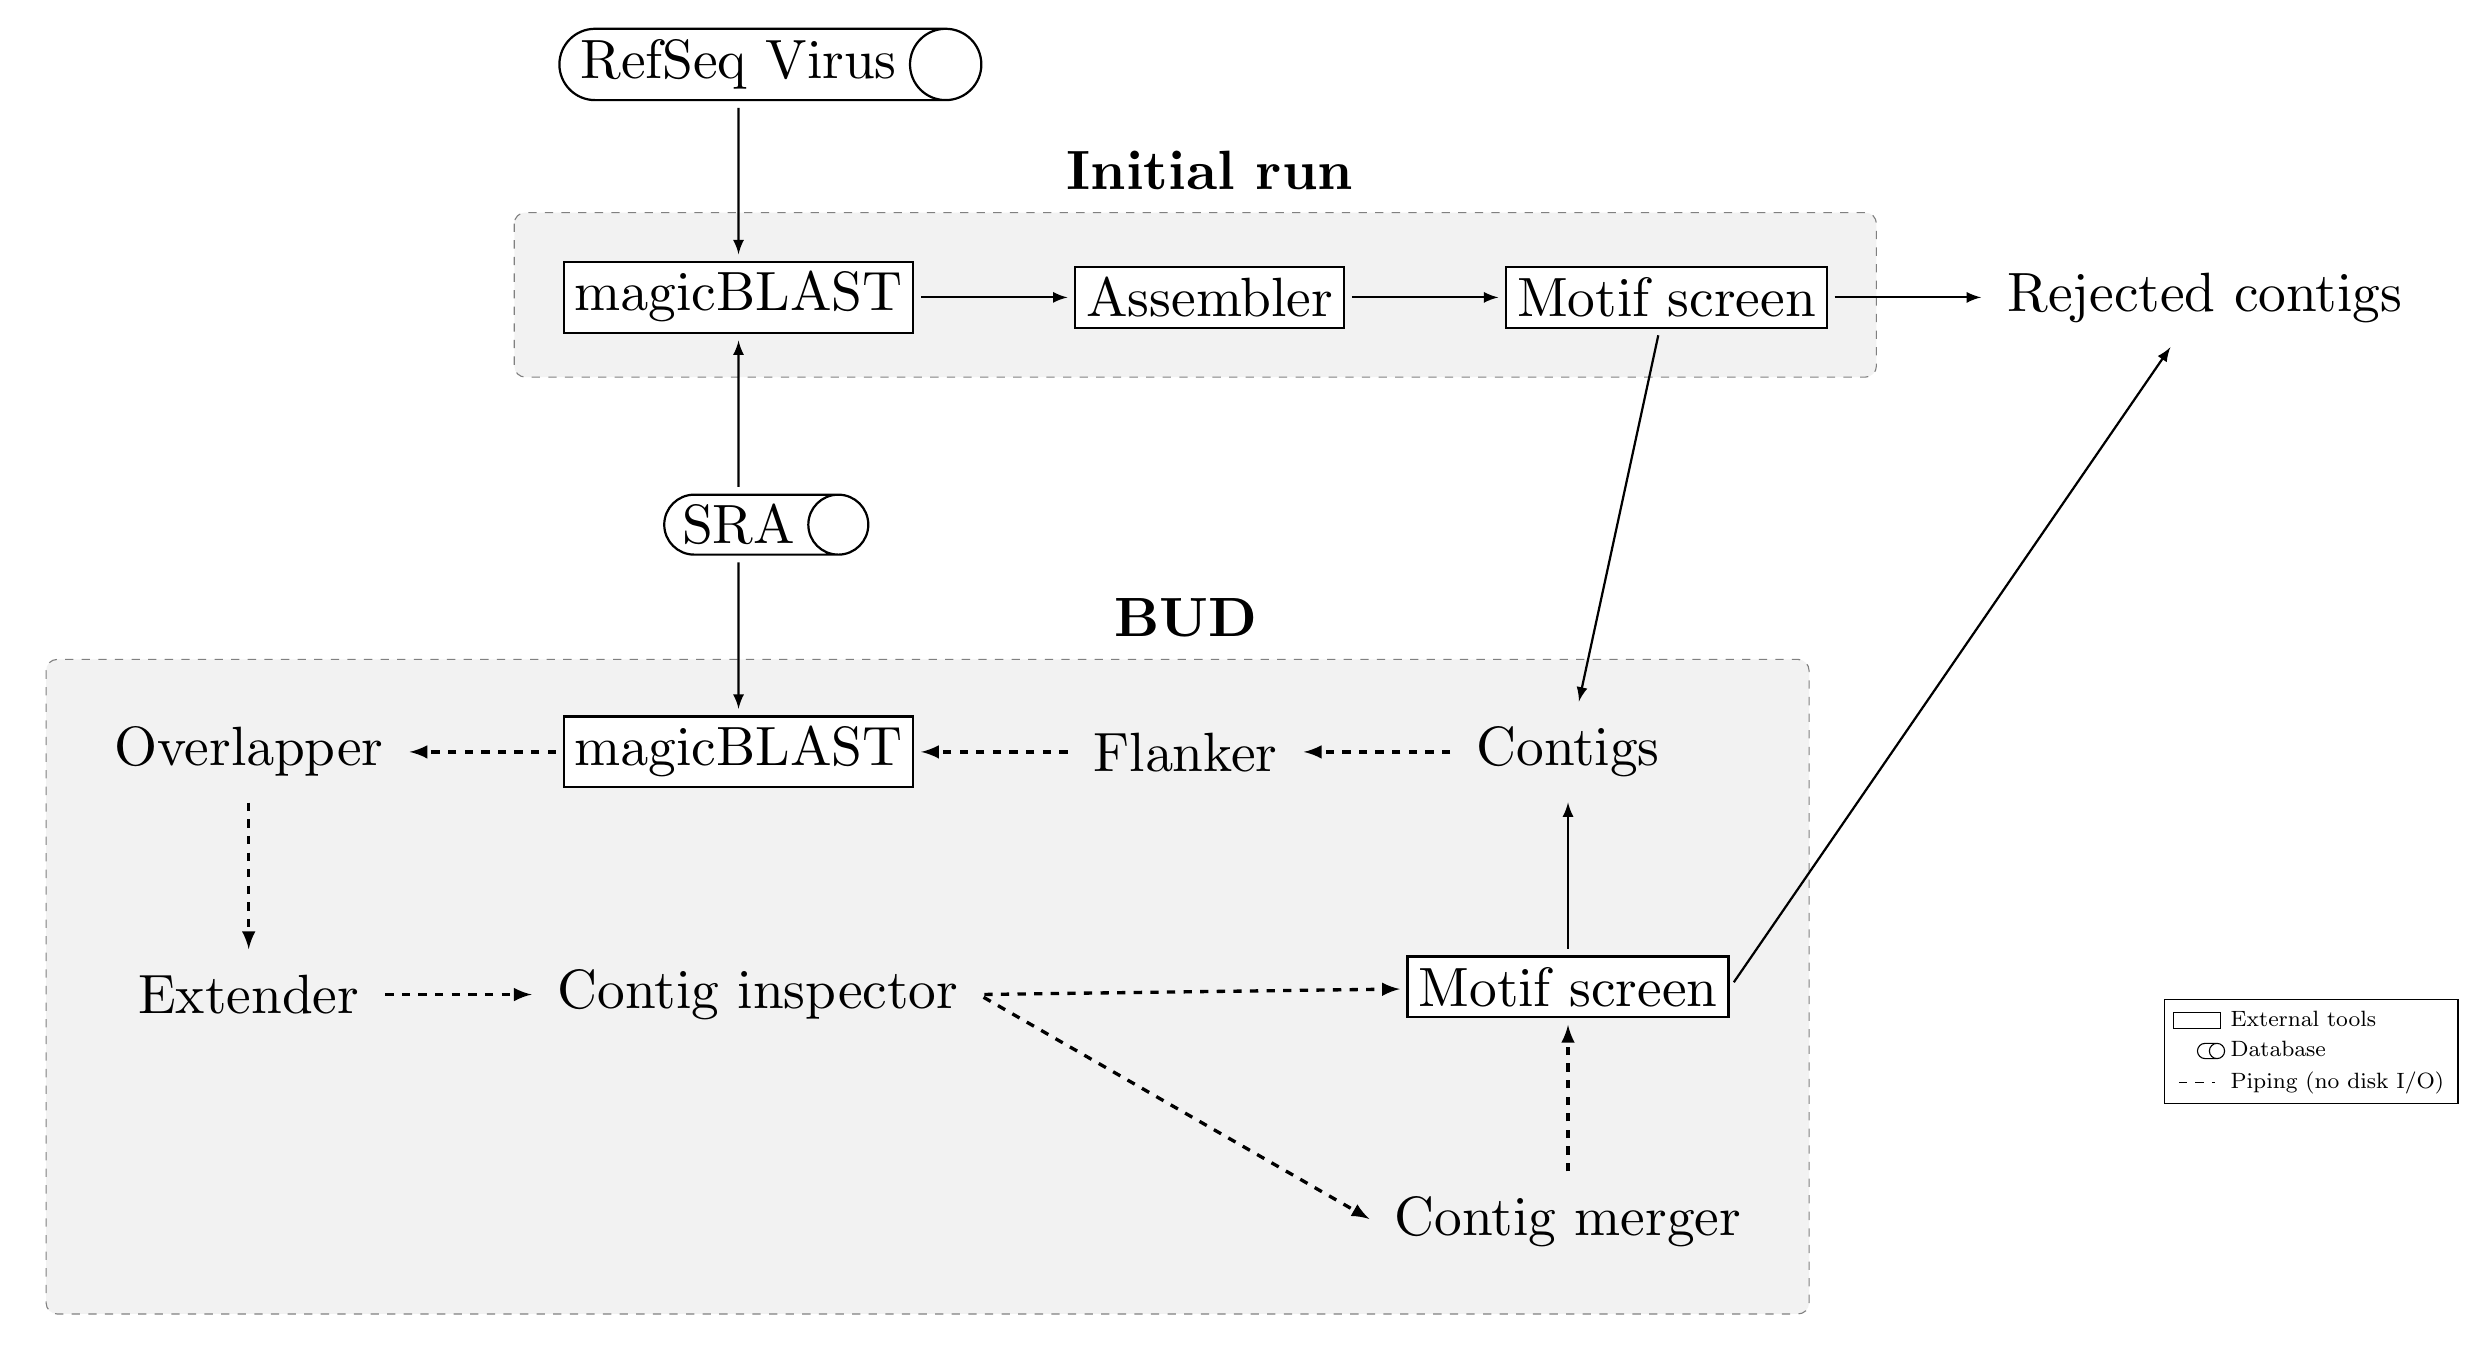
\begin{tikzpicture}[>=latex,shorten >=2pt,shorten <=2pt, thick, scale=2, every node/.style={transform shape}]
    \def\blockdist{0.3}
    \pgfdeclarelayer{background}
    \pgfdeclarelayer{foreground}
    \pgfsetlayers{background,main,foreground}

    \node (mapper)    [tool] {magicBLAST};
    \node (refseq)    [db,  above = of mapper]    {RefSeq Virus};
    \node (sra)       [db,  below = of mapper]    {SRA};
    \node (fmapper)   [tool, below = of sra]      {magicBLAST};
    \node (asm)       [tool, right = of mapper]   {Assembler};
    \node (mscreen)   [tool, right = of asm]      {Motif screen};
    \node (reject)    [data, right = of mscreen]  {Rejected contigs};
    \node (flanker)   [func, right = of fmapper]  {Flanker};
    \node (ctgs)      [data, right = of flanker]  {Contigs};
    \node (cscreen)   [tool, below = of ctgs]     {Motif screen};
    \node (overlaps)  [func, left = of fmapper]   {Overlapper};
    \node (extend)    [func, below = of overlaps] {Extender};
    \node (ctgChk)    [func, right = of extend]   {Contig inspector};
    \node (ctgMerge)  [func, below = of cscreen]  {Contig merger};


    \path[->] (refseq)    edge [path] (mapper)
              (sra)       edge [path] (mapper)
                          edge [path] (fmapper)
              (mapper)    edge [path] (asm)
              (asm)       edge [path] (mscreen)
              (mscreen)   edge [path] (reject)
                          edge [path] (ctgs)
              (ctgs)      edge [pipe] (flanker)
              (flanker)   edge [pipe] (fmapper)
              (fmapper)   edge [pipe] (overlaps)
              (overlaps)  edge [pipe] (extend)
              (extend)    edge [pipe] (ctgChk)
              (ctgChk.east)    edge [pipe] (cscreen)
                          edge [pipe] (ctgMerge.west)
              (ctgMerge)  edge [pipe] (cscreen)
              (cscreen)   edge [path] (ctgs)
              (cscreen.east)   edge [path] (reject);

    \path[partLabel] (asm.north) +(0,+2*\blockdist) node (inital_desc) {Initial run};
    \path[partLabel](flanker.north) +(0,+2*\blockdist) node (bud) {BUD};
    \begin{pgfonlayer}{background}
      \path (mapper.west |- mapper.north)+(-0.3, \blockdist) node (a) {};
      \path (mscreen.south -| mscreen.east)+(+0.3,-0.3) node (b) {};


      \path (overlaps.west |- overlaps.north)+(-0.3, \blockdist) node (c) {};
      \path (ctgMerge.south -| ctgMerge.east)+(+0.3, -0.3) node (d) {};
      \path[partLabel]
          (a) rectangle (b);
      \path[partLabel]
          (c) rectangle (d);
    \end{pgfonlayer}
    \begin{customlegend}[legend cell align=left, %<= to align cells
                         legend entries={ % <= in the following there are the entries
                                           External tools,
                                           Database,
                                           Piping (no disk I/O)},
                         legend style={at={($(d.east)+(4,2)$)},font=\footnotesize}] % <= to define position and font legend
    % the following are the "images" and numbers in the legend
        \addlegendimage{area legend}
        \addlegendimage{mark=db, draw=white}
        \addlegendimage{style=dashed, color=black}
    \end{customlegend}
  \end{tikzpicture}
\end{document}
